%\documentclass[PhD,two side]{srmuthesis}
%\documentclass[MS]{srmuthesis}
%\documentclass[MTech]{srmuthesis}
\documentclass[BTech]{srmuthesis}
\usepackage{times}
\usepackage{t1enc}
\usepackage{tikz}
\usepackage{subfigure}
\usepackage{listings}
\usepackage{color}
\usepackage{pgfplots}
\usepackage{setspace} 
\usepackage{geometry}
\usepackage{graphicx}
\usepackage{float}
\usepackage{array}
\usepackage{epstopdf}
\usepackage{lscape}
\usepackage{fancyhdr}
\usepackage{natbib}
\usepackage{hyperref} % hyperlinks for references.
\usepackage{amsmath} % easier math formulae, align, subequations \ldots
\usepackage{amssymb}
\usepackage{wasysym}
\usepackage{titlesec}
\usepackage{textcomp}
\usepackage{pifont}
\usepackage{appendix}
\usepackage{caption}
\usetikzlibrary{decorations.pathmorphing}
\usetikzlibrary{shapes,arrows,shadows,patterns}
\usepackage[printonlyused]{acronym}
%\usepackage{nomencl}
%\newcommand{\bigsize}{\fontsize{16pt}{20pt}\selectfont}
%\renewcommand\nomname{\centerline {NOTATION}}
%\makenomenclature
\setcounter{MaxMatrixCols}{20}
\captionsetup[figure]{labelfont=bf}
\begin{document}
%%%%%%%%%%%%%%%%%%%%%%%%%%%%%%%%%%%%%%%%%%%%%%%%%%%%%%%%%%%%%%%%%%%%%%
% Title page

\title{OUTLINE OF CRYPTOGRAPHY CLOUD FRAMEWORK} % Enter The Project Title

\firstauthor{ANIKET REBHANKAR }% Enter The Student name
\firstauthorregno{[Reg No: RA1511003040028]}
\secondauthor{ ALOK RANJAN }% Enter The Student name
\secondauthorregno{[Reg No: RA1511003040173]}
\thirdauthor{ FAISHAL SHAKEEL } 
\thirdauthorregno{[Reg No: RA1511003040304]}


\guide{ Mr. Ethirajulu V, B.E, M.Tech} % Enter your guide's name
\designation{Assistant Professor} % Enter your guide's designation
\guidedepartment{Computer Science \& Engg.,} % Enter the department name of your Guide 
\hod{Dr. S. PRASANNA DEVI, Ph.D} % Enter HOD's name
\department{Computer Science \& Engg.,} % Enter your department name
\date{MAY 2019} % Enter month and year of submission
%\nocite{*}

\maketitle
%%%%%%%%%%%%%%%%%%%%%%%%%%%%%%%%%%%%%%%%%%%%%%%%%%%%%%%%%%%%%%%%%%%%%%
%\vspace*{3in}
%\begin{center}
%{\Huge Dedicated to my Parents}
%\end{center}
%%%%%%%%%%%%%%%%%%%%%%%%%%%%%%%%%%%%%%%%%%%%%%%%%%%%%%%%%%%%%%%%%%%%%%
% Certificate
\certificate

%\vspace*{0.5in}



%%%%%%%%%%%%%%%%%%%%%%%%%%%%%%%%%%%%%%%%%%%%%%%%%%%%%%%%%%%%%%%%%%%%%%
% Abstract

\abstract
\begin{doublespacing}
{\large\noindent In light of the impulsive idea and volume, re-appropriating cipher texts in cloud is respected through a victor among best approaches data gathering.  A little while later, checking the course realness of a company and securely supporting a cipher text in the cloud subject to another space hypothesis allotted the data have two key endeavors to make cloud-based epic data hiding away sensible and impelling. Standard frameworks   either absolutely dismiss the issue of access structure animate or delegate the reestablish to a distant ace; paying little respect to after a short time, discover the chance to approach reinforce is fundamental for improving by company join and carelessness works. Here, we propose a checked and obvious access control imagine dependent on the cryptosystem for goliath information gathering in hazes. First propose another translating tally to beat the unscrambling frustrations of the first, and after that detail our course of action and dissect its exactness, security properties, and computational capacity. Our strategy attracts the cloud server to competently resuscitate the cipher text when another portion framework is appeared by the information proprietor, who is additionally planned to help to counter against beguiling practices of the cloud. It what's more connects with (I) the information proprietor and qualified clients to adequately recognize the authenticity of a client for getting to the information, and (ii) a client to help the data given by different clients to address plaintext recuperation. Veritable examination demonstrates that our methodology can shield qualified clients from misdirecting and ruin irrefutable strikes, for example, the procedure get.}
\end{doublespacing}

\pagebreak
%%%%%%%%%%%%%%%%%%%%%%%%%%%%%%%%%%%%%%%%%%%%%%%%%%%%%%%%%%%%%%%%%%%%%%
% Acknowledgements
\acknowledgements
Apart from the efforts of me, the success of any project depends largely on the encouragement and guidelines of many others. I take this opportunity to express my gratitude to the people who have been instrumental in the successful completion of this project. 

We place our deep sense of gratitude to our beloved {Chancellor, Our Chairman Thiru. Ravi Pachamoothoo}, for providing us with the requisite infrastructure throughout the course.

The completion of this study would have been not possible if not dependent on the steadfast support given by our {Dean (E\&T),  Dr. K. Duraivelu} and HoD/CSE, Dr. S. Prasanna Devi.

I would like to show my greatest appreciation to my {Project Coordinators Mr. D. Ajay Kumar and Mrs. Steffina}, I can't say thank you enough for the tremendous support and help offered every week when we had project discussion. Without his/her encouragement and guidance this project would not have materialized.

We are also grateful to our {guide, Mr. Ethirajulu V} for having assisted and mentored us so diligently in the process of preparing our project. Without his persistent support and cooperation, we couldn't have accomplished our ideas.

The guidance and support received from all the members who contributed and who are contributing to this project, was vital for the success of the project. I am grateful for their constant support and help.\\
%%%%%%%%%%%%%%%%%%%%%%%%%%%%%%%%%%%%%%%%%%%%%%%%%%%%%%%%%%%%%%%%%
% Table of contents etc.

\begin{singlespace}
\tableofcontents
\thispagestyle{empty}

\listoftables
\addcontentsline{toc}{chapter}{LIST OF TABLES}
\listoffigures
\addcontentsline{toc}{chapter}{LIST OF FIGURES}
\end{singlespace}


%%%%%%%%%%%%%%%%%%%%%%%%%%%%%%%%%%%%%%%%%%%%%%%%%%%%%%%%%%%%%%%%%%%%%%
\abbreviations
%\begin{acronym}[longest acronym must be entered here]
\begin{acronym}[OKID/ERA]

%\acro{acronym}{in detail}
\acro{JVM}{Java Virtual Machine}
\acro{JSP}{Java Server Page}
\acro{DSA}{Dual Sentiment Analysis}
\acro{CGI}{Common Gateway Interface}
\acro{HIBE}{Hierarchical Identity-Based Encryption}
\acro{SCA}{State Cryptography Administration}
\end{acronym}
% Use the syntax \ac{acronym} whereever you use this acronym.
% Abbreviations

%\noindent 
%\begin{tabbing}
%xxxxxxxxxxx \= xxxxxxxxxxxxxxxxxxxxxxxxxxxxxxxxxxxxxxxxxxxxxxxx \kill
%\textbf{TM}   \> Transfer Matrix \\
%\textbf{LMTM} \> Lumped Mass Transfer matrix \\
%\textbf{CMTM} \> Consistent Mass Transfer matrix \\
%\textbf{SCTM} \> Single Crack Transfer matrix \\
%\textbf{LCTM} \> Lumped Crack Transfer matrix \\
%\textbf{DCTM} \> Double Crack Transfer matrix \\
%\textbf{DOF} \> Degrees Of Freedom \\
%\textbf{GA} \> Genetic Algorithm  \\
%\textbf{PSO} \> Particle Swarm Optimization \\
%\textbf{SI} \> Structural Identification \\
%\end{tabbing}

%\pagebreak

%%%%%%%%%%%%%%%%%%%%%%%%%%%%%%%%%%%%%%%%%%%%%%%%%%%%%%%%%%%%%%%%%%%%%%
% Enter the symbols used in the thesis in alphabatical order
%\chapter*{\centerline{LIST OF SYMBOLS}}
%\addcontentsline{toc}{chapter}{LIST OF SYMBOLS}
%\nomenclature{b}{Width of the beam}
%\nomenclature{r}{Number of DOF}
%\nomenclature{n}{Number of elements}
%\nomenclature{h}{Thickness of the beam}
%\nomenclature{$\theta$}{Length of the beam}
%\nomenclature{$\omega$}{Circular frequency}
%\begin{doublespace}
%\begin{tabbing}
%%\printnomenclature
%xxxxxxxxxxx \= xxxxxxxxxxxxxxxxxxxxxxxxxxxxxxxxxxxxxxxxxxxxxxxx \kill
%\textbf{$\alpha$, $\beta$}   \> Damping constants  \\
%\textbf{$\theta$}   \> Angle of twist, rad  \\
%\textbf{$\omega$}   \> Angular velocity, rad/s  \\
%\textbf{$b$}   \> Width of the beam,  m \\
%\textbf{$h$}   \> Height of the beam,  m \\
%\textbf{$\{f(t)\}$}   \> force vector  \\
%\textbf{$[K^e]$}  \> Element stiffness matrix\\
%\textbf{$[M^e]$}  \> Element mass matrix \\
%\textbf{$\{q(t)\}$}   \> Displacement vector  \\
%\textbf{$\{\dot{q}(t)\}$}   \> Velocity vector  \\
%\textbf{$\{\ddot{q}(t)\}$}   \> Acceleration vector  \\
%
%
%\end{tabbing}
%\end{doublespace}

\pagebreak
%\clearpage
% The main text will follow from this point so set the page numbering
% to arabic from here on.
\pagenumbering{arabic}


%%%%%%%%%%%%%%%%%%%%%%%%%%%%%%%%%%%%%%%%%%%%%%%%%%
% Introduction.

%Enter your chapter number here
\chapter{INTRODUCTION}
\section{Overview of the Project}
At present, information improvement with the vivacious movement drives the musicality and pace of society. With the assistance of properties of appropriated setting up that consolidate high flexibility, high constant quality and versatility, consistently more application structures move to the cloud to pass on, for achieving the target of joined relationship of data and gifted utilization of focal core interests. Appropriated selecting improvement has been thoroughly used in the information technique for industry, record and government, which interminably supports the work and life of people; by at that point, sort out information has changed into a major thing resource, whose security can be barely considered. To ensure security of data information in the system condition, cryptography application mode under the cloudiness overseeing condition winds up being especially fundamental. The start of Crypto as a Service (Camas)] made gushed preparing from the bit of data security; it finds another course for the utilization of the cryptography development in the Cloud condition, in like way refreshes the new framework. There into, the security of cloud application is commonly about the examination on terminal mechanical get-together and framework gear kept up by trusted being made, in like seminar on the decided quality and security of re-appropriating estimations; the examination on cloud data security joins perplex, continuation, consistency and picked nature of passed on get-together data; the guaranteed research on the security of cloud hardware with the virtualization are vulnerabilities of contraption working conditions concerning virtualization, security traditions and technique for virtualized structure and security headway of cloud resource pool correspondingly as the upper virtual machine. In spite of that, Alabama Cloud influenced cloud data encryption alliance jointed JN TASS, which is to give liberal data security answers for companys that subject to contraption figure machine referenced by \ac{SCA}. So that, get a couple of information about on cloud cryptography connection that depends on working environments with virtualization work is turning up especially built develop, yet paying little personality to all that it comes up short on the cryptography organization structure with dispersed coordinating model to give cryptography affiliations.

\section{Aim of the Project}
In this paper, we propose a simple yet efficient model, called \ac{DSA}, to address the polarity shift problem in sentiment classification. By using the property that sentiment classification has two opposite class labels (i.e., positive and negative), we first propose a data expansion technique by creating sentiment reversed reviews. The original and reversed reviews are constructed in a one-to-one correspondence.



%\begin{itemize}
	%\item Medium - Ethernet devices attach to a common medium that provides a path along which the electronic signals will travel. Historically, this medium has been coaxial copper cable, but today it is more commonly a twisted pair or fiber optic cabling.
	%\item Segment - We refer to a single shared medium as an Ethernet segment.
	%\item Node - Devices that attach to that segment are stations or nodes. 
	%\item Frame - The nodes communicate in short messages called frames, which are variably sized chunks of information. 
%\end{itemize}


%Figure 1
%\begin{figure}[h]
%\centering
%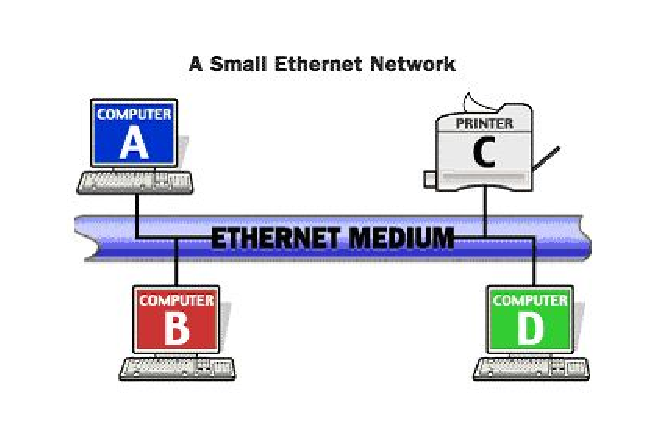
\includegraphics[width=0.9\textwidth]{Figure1.ps}
%\label{fig:1} \hspace{10mm}
%\caption{\textbf{A Small Ethernet network}}
%\end{figure}


\chapter{SYSTEM ANALYSIS}

\section{Literature Survey}
\subsection{Securing Communications Between External Users and Wireless Body Area Networks}
Remote Body Area Networks are depended upon to see a fundamental occupation in patient-achievement checking soon. Working up secure exchanges between BAN sensors and outside companys is fundamental to paying excellent character to the astonishing security and confirmation concerns. In this paper, we propose the foul abilities to regard a conundrum sharing based Cipher content Policy Attribute-Based Encryption plot, which encodes the data subject to a way structure appeared by the data source. We in like manner structure two customs to safely recuperate the unsafe patient data from a BAN and demonstrate the sensors in a BAN. Our examination demonstrates that the proposed procedure is possible, can give message validness, and can counter possible basic attacks, for instance, interest strikes and battery-weakening ambushes.
\subsection{Secure and Efficient data communication protocol for Wireless Body Area Networks}
Remote Body Area Networks are relied on to expect a key occupation in the field of patient-succeeding checking inside the not extremely far-ousted future, which increases huge idea among specialists beginning late. One of the weights is to build up a guaranteed correspondence working among sensors and clients, while paying unique personality to the outstanding security and security concerns. In this paper, we propose a correspondence sorting out for BANs, and plan a course of action to check the information exchanges between introduced/wearable sensors and the information sink/data clients (bosses or enduring pro) by using Cipher content Policy Attribute Based Encryption (CP ABE) and cutting to store the data in figure content gather at the data sink, in this way ensuring data security. Our procedure achieves an occupation based access control by using a section control tree outlined by the qualities of the information. We in like manner structure two conventions to safely recover the delicate information from a BAN and train the sensors in a BAN. We get some information about the proposed game-plan, and fight that it gives message realness and plot shirking, and is beneficial and sensible.
\subsection{Attribute-Based Encryption for Fine-Grained Access Control of Encrypted Data}
As more sensitive data is shared and stored by third-party sites on the Internet, there will be a need to encrypt data stored at these sites. One drawback of encrypting data, is that it can be selectively shared only at a coarse-grained level (i.e., giving another party your private key). We develop a new cryptosystem for fine-grained sharing of encrypted data that we call Key-Policy Attribute-Based Encryption (KPABE). In our cryptosystem, ciphertexts are labeled with sets of attributes and private keys are associated with access structures that control which ciphertexts a user is able to decrypt. We demonstrate the applicability of our construction to sharing of audit-log information and broadcast encryption. Our construction supports delegation of private keys which subsumes  \ac{HIBE}.
\subsection{Body Area Network Security: A Fuzzy Attribute-Based Signcryption Scheme}
Body Area Networks are depended upon to see a fundamental development in the field of patient-flourishing watching soon. While it is major to help secure BAN access to address the undeniable thriving and confirmation concerns, it is correspondingly primary to keep up the adaptability of such achievement endeavors. For example, flexibility is required to ensure that remedial guide staffs approach focal edifying aggregation away in a BAN in making conditions. FABSC utilize satisfying Attribute-based encryption to interface with data encryption, discover the chance to control, and moved drawing for a patient's important information in a BAN. It joins modernized etchings and encryption, and gives enigma, authenticity, enforceability, and plan square. We hypothetically exhibit that FABSC is down to earth and conceivable. We likewise separate its security level in reasonable BANs.
\subsection{An efficient threshold verifiable multi-secret sharing}
In order to fight the drive to set accommodatingly and safely, in 1979, Shamir and Blakely first developed the examinations of the issue sharing (SS) plot. The past relies upon the Lagrange embedding’s polynomial, while the prop up relies upon the direct projective geometry. In these issue sharing there are a few issues as sweeps for after: (1) In each conundrum sharing method only a particular secret can be shared; (2) These riddle sharing are the one-time-use plot, at the day's end once the puzzle has been changed, trader must redistribute another shadow over an ensured channel to each zone; (3) In them two it is standard that the vender and individuals are quick at any rate in sureness it is dazzling in the certifiable word and a confounding shipper may pass on a fake shadow to a particular part or a harmful part may give a fake arrangement to various individuals.
\section{Existing System}
In light of the impulsive idea and volume, re-appropriating cipher texts to a cloud is respected to be a victor among the best approaches for huge data gathering and get to. A little while later, checking the course realness of a company and securely supporting a cipher text in the cloud subject to another space hypothesis allotted by the data owner are two key endeavors to make cloud-based epic data hiding away sensible and impelling. Standard frameworks either absolutely dismiss the issue of access structure animate or delegate the reestablish to a distant ace; paying little respect to after a short time, discover the chance to approach reinforce is fundamental for improving security and dealing with the dynamism achieved by company join and carelessness works.




\chapter{PROPOSED METHODOLOGY}
\section{Proposed System}
Proprietor pick the item and subtleties precedent item id, item name, cost, piece, mediator name, organization name, net weight so all subtleties and abnormal state security of encryption and key likewise created, proprietor send to mediator side. Mediator client one information get so check the subtleties, the subtleties likewise encryption group so all data is print ***** as it were. Mediator client sees the first substance and downloads the item. The mediator client sends to client. Client see the message just star position so client send the solicitation so the proprietor strive the inbox and acknowledge the inquiry, client see the first information. A proficient and irrefutable technique to refresh the figure content put away in mists without expanding any hazard when the entrance strategy is progressively changed by the information proprietor for different reasons. The checking the mutual mystery data to keep clients from swindling and can counter different assaults, for example, the arrangement assault.\\
NTRU is a licensed and open source open key cryptosystem that utilizes lattice based cryptography to encode and decode information. It comprises of two calculations: NTRU Decrypt, which is utilized for Decryption, and Intrusion, which is utilized for advanced marks.

\section{Advantage of proposed system}
\textbf{•} Information proprietor and qualified clients to successfully confirm the authenticity of a client for getting to the information\\
\textbf{•} User Can Upload Secure Data .\\
\textbf{•} Corresponding to an outsider.\\

\chapter{SYSTEM IMPLEMENTATION}
In this paper, we propose a simple yet efficient model, called Clustering dual sentiment analysis (CDSA), to address the polarity shift problem in sentiment classification. By using the property that sentiment classification has two opposite class labels (i.e., positive and negative), we first propose a data expansion technique by creating sentiment reversed reviews. The original and reversed reviews are constructed in a one-to-one correspondence.\\
There are six modules for the dual sentiment analysis.

\section{Modules}
\textbf{•} User interface design \\
\textbf{•} Owner upload details and send to Mediator \\
\textbf{•} Mediator User Check Details \\
\textbf{•} Request send to owner \\
\textbf{•} Mediator send to company \\
\textbf{•} Company request send to owner \\
\section{Description}
\subsection{User interface design}
To connect with server user must give their username and password then only they can able to connect the server. If the user already exits directly can login into the server else user must register their details such as username, password and Email id, into the server. Server will create the account for the entire user to maintain upload and download rate. Name will be set as user id. Logging in is usually used to enter a specific page.
\subsection{Owner upload details and send to Mediator}
Owner choose the product and details example product id, product name, cost, piece, mediator name, company name, net weight so all details and high level security of encryption and key also developed,  owner  send to mediator side. 
\subsection{Mediator User Check Details}
Mediator user one data receive so check the details, the details also encryption format so all information is print ***** only.
\subsection{Request send to Owner} 
Mediator User view original data means send request  to data owner. The data owner monitoring the file and accept.
\subsection{Mediator send to campany}
Mediator user view the original content and download the product. The mediator user send to company.
\subsection{Company Request Send To Owner}
Company view the message only star format so company send the request so the owner view the inbox and accept the query, company view the original data.
\section{Module Diagrams}
\textbf{1. User Interface Design}
\begin{figure}[H]
\includegraphics[scale=0.7]{1.jpg}
\label{fig:1}\hspace{10mm}
\caption{\textbf{User interface diagram}}
\end{figure}
\textbf{2. Owner upload details and send to Mediator}
\begin{figure}[H]
\includegraphics[scale=0.7]{2.jpg}
\label{fig:1}\hspace{10mm}
\caption{\textbf{Owner upload details and send to Mediator}}
\end{figure}
\textbf{3. Mediator User Check Details}
\begin{figure}[H]
\includegraphics[scale=0.7]{3.jpg}
\label{fig:1}\hspace{10mm}
\caption{\textbf{Mediator User Check Details}}
\end{figure}
\textbf{4. Request send to Owner}
\begin{figure}[H]
\includegraphics[scale=0.7]{4.jpg}
\label{fig:1}\hspace{10mm}
\caption{\textbf{Request send to Owner}}
\end{figure}
\textbf{5. Mediator send to campany}
\begin{figure}[H]
\includegraphics[scale=0.7]{5.jpg}
\label{fig:1}\hspace{10mm}
\caption{\textbf{Mediator send to campany}}
\end{figure}
\textbf{6. Company Request Send To Owner}
\begin{figure}[H]
\includegraphics[scale=0.7]{6.jpg}
\label{fig:1}\hspace{10mm}
\caption{\textbf{Company Request Send To Owner}}
\end{figure}
\section{System Techniques}
An efficient and verifiable method to update the cipher text stored in clouds without increasing any risk when the access policy is dynamically changed by the data owner for various reasons. The verifying the shared secret information to prevent users from cheating and can counter various attacks such as the collusion attack.\\
NTRU is a patented and open source public-key cryptosystem that uses lattice based cryptography to encrypt and decrypt data. It consists of two algorithms: NTRU Decrypt, which is used for Decryption, which is used for digital signatures.\\

\chapter{SYSTEM REQUIREMENTS}
These are the requirements for doing the project. Without using these tools and software’s we can’t do the project. So we have two requirements to do the project.\\
1. Hardware Requirements.\\
2. Software Requirements.\\
\section{Hardware Requirements}
The hardware requirements may serve as the basis for a contract for the implementation of the system and should therefore be a complete and consistent specification of the whole system. They are used by software engineers as the starting point for the system design. It shows what the system does and not how it should be implemented.\\

\begingroup
\centering
\begin{tabular}{|c|c|}
\hline
PROCESSOR & PENTIUM IV 2.6 GHz, Intel Core 2 Duo.\\
\hline
RAM & 4GB DD RAM\\
\hline
MONITOR & 15” COLOR\\
\hline
HARD DISK & 250 GB\\
\hline
\end{tabular}
\captionof{table}{Hardware Requirement}
\label{tbl:table1}
\endgroup 
\section{Software Requirements}
The software requirements document is the specification of the system. It should include both a definition and a specification of requirements. It is a set of what the system should do rather than how it should do it. The software requirements provide a basis for creating the software requirements specification. It is useful in estimating cost, planning team activities, performing tasks and tracking the team’s and tracking the team’s progress throughout the development activity.\\

\begingroup
\centering
\begin{tabular}{|c|c|}
\hline
Front End & J2EE (JSP, SERVLETS) JAVASCRIPT\\
\hline
Back End & MY SQL 5.5 \\
\hline
Operating System & Windows 07\\
\hline
IDE & Eclipse\\
\hline
\end{tabular}
\captionof{table}{Software Requirement}
\label{tbl:table1}
\endgroup

\chapter{SYSTEM DESIGN}
Design Engineering deals with the various UML [Unified Modelling language] diagrams for the implementation of project. Design is a meaningful engineering representation of a thing that is to be built. Software design is a process through which the requirements are translated into representation of the software. Design is the place where quality is rendered in software engineering. Design is the means to accurately translate company requirements into finished product.
\section{Usecase Diagram}

\begin{figure}[H]
\centering
\includegraphics[scale=0.8]{usecase.jpg}
\label{fig:1}\hspace{10mm}
\caption{\textbf{Usecase Diagram}}
\end{figure}
The main purpose of a use case diagram shown in figure 6.1 is to show what system functions are performed for user can login and company also login.Owner choose the product and details example product id, product name, cost, piece, mediator name, company name, net weight so all details and high level security of encryption and key also developed,  owner  send to mediator side. Mediator user one data receive so check the details, the details also encryption format so all information is print ***** only.    Mediator user view the original content and download the product. The mediator user send to company. Company view the message only star format so company send the request so the owner vie the inbox and accept the query, company view the original data.\\
\section{Class Diagram}

\begin{figure}[H]
\centering
\includegraphics[scale=0.8]{class.jpg}
\label{fig:1}\hspace{10mm}
\caption{\textbf{Class Diagram}}
\end{figure}
The class diagram shown in the figure 6.2 is the main building block of object oriented modeling. It is used both for general conceptual modeling of the systematic of the application, and for detailed modeling translating the models into programming code in the Diagram we are user can login and company also login. .     Owner choose the product and details example product id, product name, cost, piece, mediator name, company name, net weight so all details and high level security of encryption and key also developed,  owner  send to mediator side. Mediator user one data receive so check the details, the details also encryption format so all information is print ***** only.    Mediator user view the original content and download the product. The mediator user send to company. Company view the message only star format so company send the request so the owner vie the inbox and accept the query, company view the original data.

\section{Object Diagram}

\begin{figure}[H]
\centering
\includegraphics[scale=0.8]{object.jpg}
\label{fig:1}\hspace{10mm}
\caption{\textbf{Object Diagram}}
\end{figure}
Object diagram shown in the figure 6.3 we are telling about the flow of objects how the process is running. In the above digram tells about the flow of objects between the classes.In the Diagram for user can login and company also login. Owner choose the product and details example product id, product name, cost, piece, mediator name, company name, net weight so all details and high level security of encryption and key also developed,  owner  send to mediator side. Mediator user one data receive so check the details, the details also encryption format so all information is print ***** only.    Mediator user view the original content and download the product. The mediator user send to company. Company view the message only star format so company send the request so the owner vie the inbox and accept the query, company view the original data.
\section{State Diagram}

\begin{figure}[H]
\centering
\includegraphics[scale=0.8]{State.jpg}
\label{fig:1}\hspace{10mm}
\caption{\textbf{State Diagram}}
\end{figure}
State diagrams shown in the figure 6.4 require that the system described is composed of a finite number of states; sometimes, this is indeed the case, while at other times this is a reasonable abstraction. Many forms of state diagrams exist, which differ slightly and have different semantics. In the Diagram for is to expose what device capabilities are performed for user can login and company also login. .     Owner choose the product and details example product id, product name, cost, piece, mediator name, company name, net weight so all details and high level security of encryption and key also developed,  owner  send to mediator side. Mediator user one data receive so check the details, the details also encryption format so all information is print ***** only. Mediator user view the original content and download the product. The mediator user send to company. Company view the message only star format so company send the request so the owner vie the inbox and accept the query, company view the original data.
\section{Sequence Diagram}

\begin{figure}[H]
\centering
\includegraphics[scale=0.9]{sequence.jpg}
\label{fig:1}\hspace{10mm}
\caption{\textbf{Sequence Diagram}}
\end{figure}
In our sequence diagram shown in the figure 6.5 specifying processes operate with one another and in order. In our sequence diagram for is to expose what device capabilities are performed for user can login and company also login. Owner choose the product and details example product id, product name, cost, piece, mediator name, company name, net weight so all details and high level security of encryption and key also developed,  owner  send to mediator side. Mediator user one data receive so check the details, the details also encryption format so all information is print ***** only. Mediator user view the original content and download the product. The mediator user send to company. Company view the message only star format so company send the request so the owner vie the inbox and accept the query, company view the original data.
\section{Data Flow Diagram}
\subsection{Level-0}

\begin{figure}[H]
\centering
\includegraphics[scale=0.8]{level0.jpg}
\label{fig:1}\hspace{10mm}
\caption{\textbf{Dataflow Level-0}}
\end{figure}
\subsection{Level-1}

\begin{figure}[H]
\centering
\includegraphics[scale=0.7]{level1.jpg}
\label{fig:1}\hspace{10mm}
\caption{\textbf{Dataflow Level-1}}
\end{figure}
\subsection{Level-2}

\begin{figure}[H]
\centering
\includegraphics[scale=0.8]{level2.jpg}
\label{fig:1}\hspace{10mm}
\caption{\textbf{Dataflow Level-2}}
\end{figure}
It does not show information about the timing of processes, or information about whether processes will operate in sequence or in parallel. In the DFDs the level zero process is based on the login validations. Owner choose the product and details example product id, product name, cost, piece, mediator name, company name, net weight so all details and high level security of encryption and key also developed,  owner  send to mediator side. Mediator user one data receive so check the details, the details also encryption format so all information is print ***** only. Mediator user view the original content and download the product. The mediator user send to company. Company view the message only star format so company send the request so the owner vie the inbox and accept the query, company view the original data.
\section{E-R Diagram}

\begin{figure}[H]
\centering
\includegraphics[scale=0.8]{er.jpg}
\label{fig:1}\hspace{10mm}
\caption{\textbf{E-R Diagram}}
\end{figure}
In the given Figure 6.9 shows the ERM diagram. Entity-Relationship Model (ERM) is an abstract and conceptual representation of data. Entity-relationship modeling is a database modeling method, used to produce a type of conceptual schema or semantic data model of a system, often a relational database. In the Diagram we show for user can login and company also login. Owner choose the product and details example product id, product name, cost, piece, mediator name, company name, net weight so all details and high level security of encryption and key also developed,  owner  send to mediator side. Mediator user one data receive so check the details, the details also encryption format so all information is print ***** only. Mediator user view the original content and download the product. The mediator user sends to company. Company view the message only star format so company send the request so the owner vie the inbox and accept the query, company view the original data.
\section{System Architecture}

\begin{figure}[H]
\centering
\includegraphics[scale=0.9]{system.jpg}
\label{fig:1}\hspace{10mm}
\caption{\textbf{System Architecture Diagram}}
\end{figure}
\section{Proposed System Model Explanation}
Owner choose the product and details example product id, product name, cost, piece, mediator name, company name, net weight so all details and high level security of encryption and key also developed,  owner  send to mediator side. Mediator user one data receive so check the details, the details also encryption format so all information is print ***** only. Mediator user view the original content and download the product. The mediator user sends to company. Company view the message only star format so company send the request so the owner vie the inbox and accept the query, company view the original data. An efficient and verifiable method to update the cipher text stored in clouds without increasing any risk when the access policy is dynamically changed by the data owner for various reasons. The verifying the shared secret information to prevent users from cheating and can counter various attacks such as the collusion attack.\\

\chapter{DEVELOPMENT TOOLS}
This chapter is about the software language and the tools used in the development of the project. The platform used here is JAVA.\\
\section{Features of Java}
\subsection{The Java Framework}
Java is a programming language originally developed by James Gosling at Microsystems and released in 1995 as a core component of Sun Microsystems' Java platform. The language derives much of its syntax from C and C++ but has a simpler object model and fewer low-level facilities. Java applications are typically compiled to bytecode that can run on any \ac{JVM} regardless of computer architecture. Java is general-purpose, concurrent, class-based, and object-oriented, and is specifically designed to have as few implementation dependencies as possible. It is intended to let application developers "write once, run anywhere".\\\\
Java is considered by many as one of the most influential programming languages of the 20th century, and is widely used from application software to web applications the java framework is a new platform independent that simplifies application development internet. Java technology's versatility, efficiency, platform portability, and security make it the ideal technology for network computing. From laptops to datacentres, game consoles to scientific supercomputers, cell phones to the Internet, Java is everywhere!\\
\subsection{Objectives of Java}
\subsubsection{Why Software Developers Choose Java}
Java has been tested, refined, extended, and proven by a dedicated community. And numbering more than 6.5 million developers, it's the largest and most active on the planet. With its versatility, efficiency, and portability, Java has become invaluable to developers by enabling them to:\\\\
1.Write software on one platform and run it on virtually any other platform.\\
2.Create programs to run within a Web browser and Web services.\\
3.Develop server-side applications for online forums, stores, polls, HTML forms processing, and more.\\
4.Combine applications or services using the Java language to create highly customized applications or services.\\
5.Write powerful and efficient applications for mobile phones, remote processors, low-cost consumer products, and practically any other device with a digital heartbeat.\\
\subsubsection{Some Ways Software Developers Learn Java}
\textbf{•} Today, many colleges and universities offer courses in programming for the Java platform. In addition, developers can also enhance their Java programming skills by reading Sun's java.sun.com Web site, subscribing to Java technology-focused newsletters, using the Java Tutorial and the New to Java Programming Center, and signing up for Web, virtual, or instructor-led courses. \\
\subsubsection{Object Oriented Language}
To be an Object Oriented language, any language must follow at least the four characteristics:-
1.Inheritance: It is the process of creating the new classes and using the behaviour of the existing classes by extending them just to reuse the existing code and adding addition a features as needed.\\
2.Encapsulation: It is the mechanism of combining the information and providing the abstraction.\\
3.Polymorphism: As the name suggest one name multiple form, Polymorphism is the way of providing the different functionality by the functions having the same name based on the signatures of the methods.\\
4.Dynamic binding: Sometimes we don't have the knowledge of objects about their specific types while writing our code. It is the way of providing the maximum functionality to a program about the specific type at runtime.\\
\subsection{Java Server Pages - An Overview}
\ac{JSP} for short is Sun's solution for developing dynamic web sites. JSP provide excellent server side scripting support for creating database driven web applications. JSP enable the developers to directly insert java code into jsp file, this makes the development process very simple and its maintenance also becomes very easy.\\\\
JSP pages are efficient, it loads into the web servers memory  on receiving the request very first time and the subsequent calls are served within a very short period of time.\\\\
In today's environment most web sites servers dynamic pages based on user request. Database is very convenient way to store the data of users and other things. JDBC provide excellent database connectivity in heterogeneous database environment. Using JSP and JDBC it’s very easy to develop database driven web application.\\\\
Java is known for its characteristic of "write once, run anywhere." JSP pages are plat Java Server Pages.Java Server Pages (JSP) technology is the Java platform technology for delivering dynamic content to web clients in a portable, secure and well-defined way. The Java Server Pages specification extends the Java Servlet API to provide web application developers with a robust framework for creating dynamic web content on the server using HTML, and XML templates, and Java code, which is secure, fast, and independent of server platforms.\\\\
JSP has been built on top of the Servlet API and utilizes Servlet semantics. JSP has become the preferred request handler and response mechanism. Although JSP technology is going to be a powerful successor to basic Servlets, they have an evolutionary relationship and can be used in a cooperative and complementary manner.\\\\
Servlets are powerful and sometimes they are a bit cumbersome when it comes to generating complex HTML. Most servlets contain a little code that handles application logic and a lot more code that handles output formatting. This can make it difficult to separate and reuse portions of the code when a different output format is needed. For these reasons, web application developers turn towards JSP as their preferred servlet environment.\\
\subsection{Evolution of Web Applications}
Over the last few years, web server applications have evolved from static to dynamic applications. This evolution became necessary due to some deficiencies in earlier web site design. For example, to put more of business processes on the web, whether in business-to-consumer (B2C) or business-to-business (B2B) markets, conventional web site design technologies are not enough. The main issues, every developer faces when developing web applications, are:\\
1. Scalability :- a successful site will have more users and as the number of users is increasing fast, the web applications have to scale correspondingly.\\
2. Integration of data and business logic :- the web is just another way to conduct business, and so it should be able to use the same middle-tier and data-access code. \\
3. Manageability :- web sites just keep getting bigger and we need some viable mechanism to manage the ever-increasing content and its interaction with business systems. \\
4. Personalization :- adding a personal touch to the web page becomes an essential factor to keep our company coming back again. Knowing their preferences, allowing them to configure the information they view, remembering their past transactions or frequent search keywords are all important in providing feedback and interaction from what is otherwise a fairly one-sided conversation.\\
Apart from these general needs for a business-oriented web site, the necessity for new technologies to create robust, dynamic and compact server-side web applications has been realized. The main characteristics of today's dynamic web server applications are as follows: \\
1. Serve HTML and XML, and stream data to the web client. \\
2. Separate presentation, logic and data. \\
3. Interface to databases, other Java applications and CORBA, directory and mail services. \\
4. Make use of application server middleware to provide transactional support. \\
5. Track client sessions.\\
\subsection{Benefits of JSP}
One of the main reasons why the Java Server Pages technology has evolved into what it is today and it is still evolving is the overwhelming technical need to simplify application design by separating dynamic content from static template display data. Another benefit of utilizing JSP is that it allows to more cleanly separate the roles of web application/HTML designer from a software developer. The JSP technology is blessed with a number of exciting benefits, which are chronicled as follows: \\\\
1. The JSP technology is platform independent, in its dynamic web pages, its web servers, and its underlying server components. That is, JSP pages perform perfectly without any hassle on any platform, run on any web server, and web-enabled application server. The JSP pages can be accessed from any web server. \\\\
2. The JSP technology emphasizes the use of reusable components. These components can be combined or manipulated towards developing more purposeful components and page design. This definitely reduces development time apart from the At development time, JSPs are very different from Servlets, however, they are precompiled into Servlets at run time and executed by a JSP engine which is installed on a Web-enabled application server such as BEA Web Logic and IBM Web Sphere.\\
\section{Servlets}
Earlier in client- server computing, each application had its own client program and it worked as a user interface and need to be installed on each user's personal computer. Most web applications use HTML/XHTML that are mostly supported by all the browsers and web pages are displayed to the client as static documents. \\ 
A web page can merely displays static content and it also lets the user navigate through the content, but a web application provides a more interactive experience. \\
Any computer running Servlets or JSP needs to have a container. A container is nothing but a piece of software responsible for loading, executing and unloading the Servlets and JSP. While servlets can be used to extend the functionality of any Java- enabled server. \\
They are mostly used to extend web servers, and are efficient replacement for \ac{CGI} scripts. \ac{CGI} was one of the earliest and most prominent server side dynamic content solutions, so before going forward it is very important to know the difference between CGI and the Servlets.\\
\section{Java Servlets}
Java Servlet is a generic server extension that means a java class can be loaded dynamically to expand the functionality of a server. Servlets are used with web servers and run inside a Java Virtual Machine (JVM) on the server so these are safe and portable. \\
Unlike applets they do not require support for java in the web browser. Unlike CGI, servlets don't use multiple processes to handle separate request. Servlets can be handled by separate threads within the same process. Servlets are also portable and platform independent.\\
A web server is the combination of computer and the program installed on it. Web server interacts with the client through a web browser. It delivers the web pages to the client and to an application by using the web browser and HTTP protocols respectively. \\
The define the web server as the package of  large number of programs installed on a computer connected to Internet or intranet for downloading the requested files using File Transfer Protocol, serving e-mail and building and publishing web pages. A web server works on a client server model.\\

\chapter{SOFTWARE TESTING}
The purpose of testing is to discover errors. Testing is the process of trying to discover every conceivable fault or weakness in a work product. It provides a way to check the functionality of components, sub assemblies, assemblies and/or a finished product It is the process of exercising software with the intent of ensuring that the Software system meets its requirements and user expectations and does not fail in an unacceptable manner. There are various types of test. Each test type addresses a specific testing requirement.
\section{Developing Methodology}
The test process is initiated by developing a comprehensive plan to test the general functionality and special features on a variety of platform combinations. Strict quality control procedures are used.\\
The process verifies that the application meets the requirements specified in the system requirements document and is bug free. The following are the considerations used to develop the framework from developing the testing methodologies.
\section{Types of Tests}
\subsection{Unit Testing}
Unit testing involves the design of test cases that validate that the internal program logic is functioning properly, and that program input produce valid outputs. All decision branches and internal code flow should be validated. It is the testing of individual software units of the application .it is done after the completion of an individual unit before integration. This is a structural testing, that relies on knowledge of its construction and is invasive. Unit tests perform basic tests at component level and test a specific business process, application, and/or system configuration. Unit tests ensure that each unique path of a business process performs accurately to the documented specifications and contains clearly defined inputs and expected results.
\subsection{Functional test}
Functional tests provide systematic demonstrations that functions tested are available as specified by the business and technical requirements, system documentation, and user manuals.\\
Functional testing is centered on the following items:\\
Valid Input : identified classes of valid input must be accepted.\\
Invalid Input : identified classes of invalid input must be rejected.\\
Functions : identified functions must be exercised.\\
Output : identified classes of application outputs must be exercised.\\
Systems/Procedures : interfacing systems or procedures must be invoked.
\subsection{System Test}
System testing ensures that the entire integrated software system meets requirements. It tests a configuration to ensure known and predictable results. An example of system testing is the configuration oriented system integration test. System testing is based on process descriptions and flows, emphasizing pre-driven process links and integration points.
\subsection{Performance Test}
The Performance test ensures that the output be produced within the time limits,and the time taken by the system for compiling, giving response to the users and request being send to the system for to retrieve the results.
\subsection{Integration Testing}
Software integration testing is the incremental integration testing of two or more integrated software components on a single platform to produce failures caused by interface defects.\\\\
The task of the integration test is to check that components or software applications, e.g. components in a software system or – one step up – software applications at the company level – interact without error.
\subsection{Acceptance Testing}
User Acceptance Testing is a critical phase of any project and requires significant participation by the end user. It also ensures that the system meets the functional requirements.\\
\textbf{Acceptance testing for Data Synchronization:}\\
\textbf{•} The Acknowledgements will be received by the Sender Node after the Packets are received by the Destination Node.\\
\textbf{•} The Route add operation is done only when there is a Route request in need.\\
\textbf{•} The Status of Nodes information is done automatically in the Cache Updation process.
\subsection{Build the test plan}
Any project can be divided into units that can be further performed for detailed  processing. Then a testing strategy for each of this unit is carried out. Unit testing helps to identity the possible bugs in the individual component, so the component that has bugs can be identified and can be rectified from errors.









\chapter{Results and Discussion}
\section{Results}
When the Owner, register and log-in into the account and uploads the product details like product id, product name, cost, piece, Customer name, company name and  net weight so all details and high level security of encryption and key also get developed,and owner shares details to Mediator. 
\begin{figure}[H]
\centering
\includegraphics[width=0.7\textwidth]{Ownerviewpage.jpg}
\label{Figure:10} \hspace{10mm}
\caption{\textbf{Owner-View Page}}
\end{figure}
Owner accepts the request from the Mediator and the Campany.
\begin{figure}[H]
\centering
\includegraphics[width=0.7\textwidth]{filerequestacceptpage.jpg}
\label{Figure:10} \hspace{10mm}
\caption{\textbf{File-Request Acceptance Page}}
\end{figure}
This is the Mediator's-Inbox where Mediator could get all the  Product details from the owner. In this Inbox, the Mediator does not have any access to edit the product details which is provided by the owner. The mediator could able to download the product details and can also able to share the details with the Company.
\begin{figure}[H]
\centering
\includegraphics[width=0.7\textwidth]{mediatorinboxpage.jpg}
\label{Figure:10} \hspace{10mm}
\caption{\textbf{Mediator-Inbox Page}}
\end{figure}

\begin{figure}[H]
\centering
\includegraphics[width=0.7\textwidth]{companyinbox.jpg}
\label{Figure:10} \hspace{10mm}
\caption{\textbf{Company-Inbox Page}}
\end{figure}
In the Company-Inbox, the Company could only receive the product details which are shared by the Mediator. The received details are in encrypted format like"****". To view that details the Campany can request the owner to decrypt it. When the request gets allowed from the owner's side, then only the Company could be able to view and download the Product details.

\chapter{CONCLUSION AND FUTURE ENHANCEMENT}

\section{CONCLUSION}
In this project, we propose the discharging disappointments of the first and after that present a certified and certain way control plot subject to the improved to guarantee the redistributed colossal educational record away in a cloud. Our strategy crushes in the information proprietor to immovably proceed with the information discover the chance to structure and the cloud server to sensibly restore the disconnecting re-appropriated figure content with attract solid access request over the enormous information in the cloud. It other than gives an underwriting structure to a client to help its validness of getting to the information to both the information proprietor and other ensured clients and the rightness of the data given by the t1 certain clients for plaintext recuperation. We have completely restricted the precision, security quality and computational difficult to miss examinations of our proposed procedure. Dealing with a guaranteed, security ensuring and reasonable conceptualizes for mammoth data conglomerating in a cloud is a strikingly troublesome issue. 

\section{FUTURE ENHANCEMENTS}
The security issues when an information proprietor re-appropriates its information to multi cloud servers and consider a quality based access structure   that should be capability associated with, which consistently material for sensible conditions in enormous data is putting away. Dealing with a guaranteed, affirmations guaranteeing and sensible make for enormous data checking in a cloud.

%verbatim
%%%%%%%%%%%%%%%%%%%%%%%%%%%%%%%%%%%%%%%%%%%%%%%%%%%%%%%%%%%%%
%% ANHÄNGE
%%%%%%%%%%%%%%%%%%%%%%%%%%%%%%%%%%%%%%%%%%%%%%%%%%%%%%%%%%%%%
\appendix
%% ==> Schreiben Sie hier Ihren Text oder fügen Sie externe Dateien ein.
\chapter{SAMPLE CODING}
\textbf{1. UserRegister.jsp:-}
\begin{verbatim}
<%@page language="java" contentType="text/html; 
charset=ISO-8859-1"
pageEncoding="ISO-8859-1"%>
<html lang="en">
<head>
<meta charset="utf-8">
<title>CLOUD COMPUTING</title> 
<meta name="description" content="" />
<meta name="keywords" content="" />
<meta name="viewport" content="width=device-width
, initial-scale=1.0, maximum-scale=1.0" />
<link rel="stylesheet" type="text/css"
  media="all" href="css/metro.css" />
<script src="http://ajax.googleapis.com/ajax/
libs/jquery/1.9.1/jquery.min.js"></script>
<script src="js/jquery.plugins.min.js"></script>
<script src="js/metro.js"></script>
</head> 
<body>
<div class="metro-layout horizontal">
	<div class="header">
			<h1>CLOUD COMPUTING</h1>
			<div class="controls">
<span class="down" title="Scroll down"></span>
<span class="up" title="Scroll up"></span>
<span class="next" title="Scroll left"></span>
<span class="prev" title="Scroll right"></span>
<span class="toggle-view" title="Toggle layout"></span>
</div>
</div>
<div class="content clearfix">
<div class="items">
<a class="box" href="Register.jsp">
<span>User Register</span>
<img class="icon" src="images/businessman (1).png" alt="" />
</a>
<a class="box" href="company.jsp"
 style="background: #6b6b6b;">
<span>Company</span>
<img class="icon" src="images/
icons8-Under Computer-48.png" alt="" />
</a>
<a class="box" href="#" style="background: #3c5b9b;">
<a class="box" href="Login.jsp" 
style="background: #f58d00;">
<span>Login</span>
<img class="icon" src="images/icons8-Logout
 Rounded Up-64.png" alt="" />
</a>
<a class="box" href="mediator.jsp" 
style="background: #00aeef;">
<span>Mediator User</span>
<img class="icon" src="images/
icons8-Collaborator Male-48.png" alt="" />
</a>
<a class="box height2" href="#" 
style="background: #d32c2c;">
<span>Contact</span>
<img class="icon" src="images/phone.png" alt="" />
</a>
<html lang="en" class="no-js">
<head>
<title>LOGIN</title>
<meta charset="utf-8">
<meta name="viewport" content="width=device-width
, initial-scale=1">
<link href='http://fonts.googleapis.com/
css?family=Montserrat:300,400,
700' rel='stylesheet' type='text/css'>
	<link href='https://fonts.googleapis.com/
	css?family=Raleway:400,300,500,600,700'
	 rel='stylesheet' type='text/css'>
	<link href='https://fonts.googleapis.com/
	css?family=Droid+Serif:400,400italic'
	 rel='stylesheet' type='text/css'>
<link rel="stylesheet" type="text/css" href="css/
bootstrap.min.css" media="screen">	
<link rel="stylesheet" type="text/css" href="css/
owl.carousel.css" media="screen">
<link rel="stylesheet" type="text/css" href="css/
owl.theme.css" media="screen">
<link rel="stylesheet" type="text/css" href="css/
font-awesome.css" media="screen">
<link rel="stylesheet" type="text/css" href="css/
style.css" media="screen">
<link rel="stylesheet" href="css/style1.css">
  <link rel="stylesheet" href="css/set1.css">

  <!--Google Fonts-->
  <link href='https://fonts.googleapis.com/
  css?family=Playfair+Display' 
  rel='stylesheet' type='text/css'>
  <link href='https://fonts.googleapis.com/
  css?family=Lato:400,700'
   rel='stylesheet' type='text/css'>

</head>
<body>
<section class="page-banner-section">
<div class="container">
<h1 style="float: left;">REGISTER PAGE</h1>
</div>
</section>
<div id="main-wrapper">
<div class="container-fluid">
    <div class="row">
      <div class="col-md-6 left-side">
        <header>
          <span>Need an account?</span>
          <h3>Create Account<br>Make Profits</h3>
        </header>
      </div>
<form action="Register" method="post">
<div class="col-md-6 right-side">
span class="input input--hoshi">
<input class="input__field input__field--hoshi" 
type="text" id="Username" title="Username 
(letters and numbers only, no punctuation or
 special characters)" pattern="[A-Za-z0-9]+" 
   name="Username"  required="required"/>
 <label class="input__label input__label--hoshi
  input__label--hoshi-color-3" for="Username">
<span class="input__label-content
 input__label-content--hoshi">Name</span>
          </label>
        </span>
<span class="input input--hoshi">
<input class="input__field input__field--hoshi"
 type="text" id="email" name="email" pattern="
 [a-z0-9._%+-]+@[a-z0-9.-]+\.[a-z]{2,3}$"
title="Please enter valid email address"  required="required" />
<label class="input__label input__label--hoshi
 input__label--hoshi-color-3" for="email">
<span class="input__label-content input_
_label-content--hoshi">E-mail</span>
</label>
</span>
<span class="input input--hoshi">
<input class="input__field input__field--hoshi"
 type="password" id="password" pattern="(?=.*\d)(?=.*[a-z])
 (?=.*[A-Z]).{8,}" title="Must contain at least one number
  and one uppercase and lowercase letter, and at
   least 8 or more characters" 
    name="password" required="required"/>
<label class="input__label input__label--hoshi
 input__label--hoshi-color-3" for="password">
            <span class="input__label-content
 input__label-content--hoshi">Password</span>
          </label>
        </span>
          </label>
        </span>
 
        <div class="cta">
<button class="btn btn-primary pull-left">
            Sign-Up Now
          </button>
<span><a href="Login.jsp">I am already a member</a></span> 
        </div>
package com.servlet;
import java.io.IOException;
import javax.servlet.ServletException;
import javax.servlet.annotation.WebServlet;
import javax.servlet.http.HttpServlet;
import javax.servlet.http.HttpServletRequest;
import javax.servlet.http.HttpServletResponse;
import javax.servlet.http.HttpSession;
import com.bean.Bean;
import com.imple.Imple;
import com.inter.Inter;
import com.servlet.*;
@WebServlet("/Register")
public class Register extends HttpServlet {
	private static final long serialVersionUID = 1L;
    public Register() {
        super();
        // TODO Auto-generated constructor stub
    }
	protected void doGet(HttpServletRequest request,
	 HttpServletResponse response)
	  throws ServletException, IOException {
		// TODO Auto-generated method stub
	}
	protected void doPost(HttpServletRequest request,
	 HttpServletResponse response)
	  throws ServletException, IOException {
String Username=request.getParameter("Username");
String email=request.getParameter("email");
String password=request.getParameter("password");
String Confirmpassword=request.getParameter("Confirmpassword");
String Mobile=request.getParameter("Mobile");
HttpSession session=request.getSession();
response.getContentType();
session.setAttribute("Username", Username);
System.out.println("Confirmpassword"+Confirmpassword);
Bean rb=new Bean();
rb.setUsername(Username);
rb.setEmail(email);
rb.setPassword(password);
rb.setConfirmpassword(Confirmpassword);
rb.setMobile(Mobile);
Inter asd= new Imple();
int i=asd.register(rb);
		if(i==1){
			response.sendRedirect("Login.jsp");
		}                          
		else{
			response.sendRedirect("Error.jsp");
		}}}        
\end{verbatim}
\textbf{2. Fileupload.jsp:-}
\begin{verbatim}
<%@ page import="com.servlet.Login" %>
<%@ page import="java.util.*" %>

<html lang="en" class="no-js">
<head>
	<title>LOGIN</title>

<meta charset="utf-8">
<meta name="viewport" content="width=device-width,
 initial-scale=1">

<link href='http://fonts.googleapis.com/css?
family=Montserrat:300,400,700'
 rel='stylesheet' type='text/css'>
	<link href='https://fonts.googleapis.com/
	css?family=Raleway:400,300,500,600,700'
	 rel='stylesheet' type='text/css'>
	<link href='https://fonts.googleapis.com/
	css?family=Droid+Serif:400,400italic'
	 rel='stylesheet' type='text/css'>
	
	
<link rel="stylesheet" type="text/css"
 href="css/bootstrap.min.css" media="screen">	
<link rel="stylesheet" type="text/css"
 href="css/owl.carousel.css" media="screen">
<link rel="stylesheet" type="text/css"
 href="css/owl.theme.css" media="screen">
<link rel="stylesheet" type="text/css" 
href="css/font-awesome.css" media="screen">
<link rel="stylesheet" type="text/css"
 href="css/style.css" media="screen">
<link rel="stylesheet" href="css/style1.css">
  <link rel="stylesheet" href="css/set1.css">
  <link href='https://fonts.googleapis.com/
  css?family=Playfair+Display' 
  rel='stylesheet' type='text/css'>
  <link href='https://fonts.googleapis.com/
  css?family=Lato:400,700'
   rel='stylesheet' type='text/css'>
</head>
<body>
<%Random r= new Random(); 
String key="ABCDEF123456789";
char c=key.charAt(r.nextInt(key.length()));
char c1=key.charAt(r.nextInt(key.length()));
char c2=key.charAt(r.nextInt(key.length()));
char c3=key.charAt(r.nextInt(key.length()));
char c4=key.charAt(r.nextInt(key.length()));
char c5=key.charAt(r.nextInt(key.length()));
String Secretkey=""+c+""+c1+""+c2+""+c3+""+c4+""+c5;
System.out.print(Secretkey);
HttpSession session2=request.getSession();
session.setAttribute( "key",Secretkey);%>
<section class="page-banner-section">
			<div class="container">
<h1 style="float: left;">FILE UPLOAD PAGE</h1>
			</div>
		</section>
		
		<div id="main-wrapper">

  <div class="container-fluid">
    <div class="row">
      <div class="col-md-6 left-side">
        <header>
          <span>Need an account?</span>
          <h3>Create Account<br>Make Profits</h3>
        </header>
      </div>
<form action="Upload"
 method="post" enctype="multipart/form-data">
      <div class="col-md-6 right-side">
        <span class="input input--hoshi">
<input class="input__field input__field--hoshi"
 type="text" id="productid"  name="productid" 
 required="required"/>
  <label class="input__label input__label--hoshi 
  input__label--hoshi-color-3" for="productid">
            <span class="input__label-content
             input__label-content--hoshi">PRODUCTID</span>
          </label>
        </span>
        <span class="input input--hoshi">
          <input class="input__field input__field
          --hoshi" type="text" id="productname"
           name="productname" required="required" />
          <label class="input__label input__label-
  -hoshi input__label--hoshi-color-3" for="productname">
            <span class="input__label-content
             input__label-content--hoshi">PRODUCTNAME</span>
          </label>
        </span>
        <span class="input input--hoshi">
          <input class="input__field input__field
          --hoshi" type="text" id="cost"  name
          ="cost" required="required"/>
          <label class="input__label input__label-
          -hoshi input__label--hoshi-color-3" for="cost">
            <span class="input__label-content input
            __label-content--hoshi">COST</span>
          </label>
        </span>
        <span class="input input--hoshi">
          <input class="input__field input__field-
          -hoshi" type="text" id="netweight" name
          ="netweight" required="required" />
          <label class="input__label input__label
     --hoshi input__label--hoshi-color-3" for="netweight">
            <span class="input__label-content input
            __label-content--hoshi">NETWEIGHT</span>
          </label>
        </span>
 
        <span class="input input--hoshi">
          <input class="input__field input__field
          --hoshi" type="text" id="expirydate" 
          name="expirydate" required="required" />
          <label class="input__label input__label
          --hoshi input__label--
          hoshi-color-3" for="expirydate">
            <span class="input__label-content 
            input__label-content--hoshi">EXPIRYDATE</span>
          </label>
        </span>
        <span class="input input--hoshi">
          <input class="input__field input__field--hoshi"
           type="text" id="maxpieces" 
           name="maxpieces" required="required" />
          <label class="input__label input__label
          --hoshi input__label-
          -hoshi-color-3" for="maxpieces">
            <span class="input__label-content 
            input__label-content--hoshi">MAXPIECES</span>
          </label>
        </span>
 <span class="input input--hoshi">
  <input class="input__field input__field-
   -hoshi" type="text" id="customsname"
    name="customsname" required="required" />
   <label class="input__label input__label-
   -hoshi input__label-
   -hoshi-color-3" for="customsname">
    <span class="input__label-content
    input__label-content--hoshi">CUSTOMSNAME</span>
  </label>
    </span>
       <span class="input input--hoshi">
      <input class="input__field input__field-
     -hoshi" type="text" id="company" name=
     "company" required="required" />
     <label class="input__label input__label
     --hoshi input__label--hoshi-color-3" for="company">
       <span class="input__label-content 
      input__label-content--hoshi">COMPANY</span>
      </label>
     </span>
    <span class="input input--hoshi">
    <input class="input__field input__field--hoshi"
type="text" id="country" 
name="country" required="required" />
 <label class="input__label input__label
 --hoshi input__label--hoshi-color-3" for="country">
  <span class="input__label-content
   input__label-content--hoshi">COUNTRY</span>
   </label>
    <span>
   <h5>File Secret Key:</h5><input type="text"
    readonly="readonly" name="secretkey" 
     value="<%=Secretkey%>"/><br> <br>
    <input type="file" name="file"> <br> <br>
    <div class="cta">
     <button class="btn btn-primary pull-left">
           Upload Now
          </button>
package com.servlet;
import java.io.File;
import java.io.FileInputStream;
import java.io.FileNotFoundException;
import java.io.FileOutputStream;
import java.io.IOException;
import java.io.InputStream;
import java.io.OutputStream;
import java.security.InvalidKeyException;
import java.security.NoSuchAlgorithmException;
import javax.crypto.BadPaddingException;
import javax.crypto.Cipher;
import javax.crypto.IllegalBlockSizeException;
import javax.crypto.KeyGenerator;
import javax.crypto.NoSuchPaddingException;
import javax.crypto.SecretKey;
public class EncryptFile {
KeyGenerator keyGenerator = null;
    SecretKey secretKey = null;
    Cipher cipher = null;
public EncryptFile() {
        try {
   keyGenerator = KeyGenerator.getInstance("Blowfish");
   secretKey = keyGenerator.generateKey();
   cipher = Cipher.getInstance("Blowfish");
        } catch (NoSuchPaddingException ex) {
            System.out.println(ex);
        } catch (NoSuchAlgorithmException ex) {
            System.out.println(ex);
        }
    }

    public static void main(String[] args) {
        String fileToEncrypt = "fileToEncrypt.jpg";
        String encryptedFile = "encryptedFile.jpg";
        String decryptedFile = "decryptedFile.jpg";
String directoryPath = "C:/Users/Desktop/blowfish/";
        String editPath="D:\\eclipse [JUNO]\\";
		System.out.println(editPath);
String fullpath=editPath+"Im07\\WebContent\\local\\";
String EncFile=editPath+"Im07\\WebContent\\EncryptFile\\";
EncryptFile encryptFile = new EncryptFile();
System.out.println("Starting Encryption...");
encryptFile.encrypt(directoryPath + fileToEncrypt,
                directoryPath + encryptedFile);
        System.out.println("Encryption completed...");
        System.out.println("Starting Decryption...");
        encryptFile.decrypt(EncFile + encryptedFile,
        		fullpath + decryptedFile);
        System.out.println("Decryption completed...");
    }
    public void encrypt(String srcPath, String destPath) {
        File rawFile = new File(srcPath);
        File encryptedFile = new File(destPath);
        InputStream inStream = null;
        OutputStream outStream = null;
        try {
           
            cipher.init(Cipher.ENCRYPT_MODE, secretKey);
            inStream = new FileInputStream(rawFile);
            outStream = new FileOutputStream(encryptedFile);
            byte[] buffer = new byte[1024];
            int len;
            while ((len = inStream.read(buffer)) > 0) {
                outStream.write(cipher.update(buffer, 0, len));
                outStream.flush();
            }
            outStream.write(cipher.doFinal());
            inStream.close();
            outStream.close();
        } catch (IllegalBlockSizeException ex) {
            System.out.println(ex);
        } catch (BadPaddingException ex) {
            System.out.println(ex);
        } catch (InvalidKeyException ex) {
            System.out.println(ex);
        } catch (FileNotFoundException ex) {
            System.out.println(ex);
        } catch (IOException ex) {
            System.out.println(ex);
        }
    }
    public void decrypt(String srcPath, String destPath) {
    	

String editPath="D:\\eclipse [JUNO]\\";
System.out.println(editPath);
String fullpath=editPath+"Im07\\WebContent\\local\\";
String EncFile=editPath+"Im07\\WebContent\\EncryptFile\\";
File encryptedFile = new File(EncFile);
File decryptedFile = new File(fullpath);
InputStream inStream = null;
OutputStream outStream = null;
try {
     cipher.init(Cipher.DECRYPT_MODE, secretKey);
     inStream = new FileInputStream(encryptedFile);
    outStream = new FileOutputStream(decryptedFile);
    byte[] buffer = new byte[1024];
    int len;
    while ((len = inStream.read(buffer)) > 0) 
    outStream.write(cipher.update(buffer, 0, len));
    outStream.flush();
            }
            outStream.write(cipher.doFinal());
            inStream.close();
            outStream.close();
        } catch (IllegalBlockSizeException ex) {
            System.out.println(ex);
        } catch (BadPaddingException ex) {
            System.out.println(ex);
        } catch (InvalidKeyException ex) {
            System.out.println(ex);
        } catch (FileNotFoundException ex) {
            System.out.println(ex);
        } catch (IOException ex) {
            System.out.println(ex);
        }
     }
  }
        
        
        protected void doPost(HttpServletRequest request,
 HttpServletResponse response) throws ServletException,
  IOException {String Username=request.getParameter("Username");
		String email=request.getParameter("email");
		String password=request.getParameter("password");
		String Confirmpassword=request.getParameter("Confirmpassword");
		String Mobile=request.getParameter("Mobile");
		HttpSession session=request.getSession();
		response.getContentType();
		session.setAttribute("Username", Username);
		System.out.println("Confirmpassword"+Confirmpassword);
		Bean rb=new Bean();
		rb.setUsername(Username);
		rb.setEmail(email);
		rb.setPassword(password);
		rb.setConfirmpassword(Confirmpassword);
		rb.setMobile(Mobile);
		
		Inter asd= new Imple();
		int i=asd.register(rb);
		if(i==1){
			response.sendRedirect("Login.jsp");
		}                          
		else{
			response.sendRedirect("Error.jsp");
		}}}
\end{verbatim}

\chapter{SCREENSHOTS}

\begin{figure}[H]
\centering
\includegraphics[width=0.9\textwidth]{homepage.jpg}
\label{Figure:10} \hspace{10mm}
\caption{\textbf{Homepage}}
\end{figure}

\begin{figure}[H]
\centering
\includegraphics[width=0.9\textwidth]{registerpage.jpg}
\label{Figure:10} \hspace{10mm}
\caption{\textbf{Register Page}}
\end{figure}

\begin{figure}[H]
\centering
\includegraphics[width=0.9\textwidth]{loginpage.jpg}
\label{Figure:10} \hspace{10mm}
\caption{\textbf{Login Page}}
\end{figure}

\begin{figure}[H]
\centering
\includegraphics[width=0.9\textwidth]{filepage.jpg}
\label{Figure:10} \hspace{10mm}
\caption{\textbf{File Upload Page}}
\end{figure}

\begin{figure}[H]
\centering
\includegraphics[width=0.9\textwidth]{Ownerviewpage.jpg}
\label{Figure:10} \hspace{10mm}
\caption{\textbf{Owner View Page}}
\end{figure}

\begin{figure}[H]
\centering
\includegraphics[width=0.9\textwidth]{filerequestacceptpage.jpg}
\label{Figure:10} \hspace{10mm}
\caption{\textbf{File Request Acceptance Page}}
\end{figure}

\begin{figure}[H]
\centering
\includegraphics[width=0.9\textwidth]{ownersharepage.jpg}
\label{Figure:10} \hspace{10mm}
\caption{\textbf{Owner Share Page}}
\end{figure}

\begin{figure}[H]
\centering
\includegraphics[width=0.9\textwidth]{filesharestatus.jpg}
\label{Figure:10} \hspace{10mm}
\caption{\textbf{File Share Status}}
\end{figure}

\begin{figure}[H]
\centering
\includegraphics[width=0.9\textwidth]{mediatorinboxpage.jpg}
\label{Figure:10} \hspace{10mm}
\caption{\textbf{Mediator Inbox Page}}
\end{figure}

\begin{figure}[H]
\centering
\includegraphics[width=0.9\textwidth]{mediatorsharepage.jpg}
\label{Figure:10} \hspace{10mm}
\caption{\textbf{Mediator Share Page}}
\end{figure}

\begin{figure}[H]
\centering
\includegraphics[width=0.9\textwidth]{companyinbox.jpg}
\label{Figure:10} \hspace{10mm}
\caption{\textbf{Company Inbox Page}}
\end{figure}

\begin{figure}[H]
\centering
\includegraphics[width=0.9\textwidth]{logoutpage.jpg}
\label{Figure:10} \hspace{10mm}
\caption{\textbf{Logout Page}}
\end{figure}



%%%%%%%%%%%%%%%%%%%%%%%%%%%%%%%%%%%%%%%%%%%%%%%%%%%%%%%%%%%%
% Bibliography.

\begin{singlespace}
  \bibliography{thesis_refer} % Enter your .bib file name here
  \cite{cd}\\
 \cite{bc}\\
 \cite{as}\\
 \cite{sd}\\
 \cite{aq}\\
 \cite{aw}\\
  \cite{ad}\\
  \cite{ae}\\
  \cite{at}\\
  \cite{sw}\\
  \cite{de}\\
  \cite{er}\\
  \cite{tr}\\
  \cite{fd}\\
\end{singlespace}
%%%%%%%%%%%%%%%%%%%%%%%%%%%%%%%%%%%%%%%%%%%%%%%%%%%%%%%%%%%%
  \end{document}
